%----------------------------------------------------------------------------------------
%    INTERFÈNCIA I DIFRACCIÓ
%----------------------------------------------------------------------------------------
\section{Interferència i difracció}
\subsection{Diferència de fase i coherència}
Quan dues ones harmòniques de la mateixa freqüència i longitud se superposen, tenim:
\begin{align}
    \boxed{I_{T} = I_{1} + I_{2} + 2 \sqrt{I_{1} I_{2}} \cos \delta}
\end{align}

i $\delta$, la diferència de fase deguda a una diferència de camins, ve donada per:
\begin{align}
    \boxed{\delta = k \Delta r = \frac{2 \pi}{\lambda} \Delta r}
\end{align}
Si $\delta = 2 \pi m$, tenim una interferència constructiva. En canvi, si és $\delta = (2m-1) \pi$, és destructiva. ($m \in \mathbb{N}$).

Quan una ona és reflectida en una superfície d'un medi pel qual viatja més lentament, es produeix un canvi de fase de la llum reflectida de $\boxed{\delta_{R} = \pi}$.

%----------------------------------------------------------------------------------------
\subsection{Interferència en làmines primes}
\begin{figure}[H]
\centering
    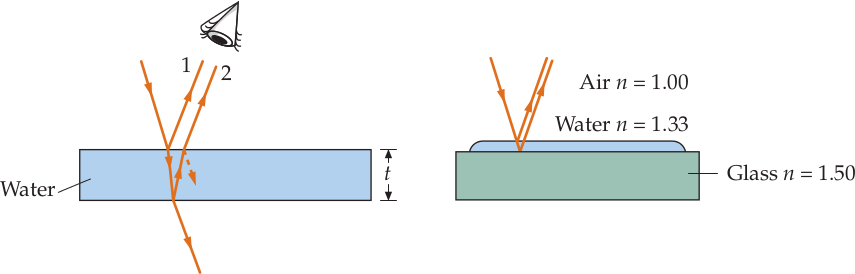
\includegraphics[width=0.9\textwidth]{images/6/62-lamines.png}
\caption{Diagrama de rajos que impacten en làmines primes}
\end{figure}
A més de la diferència de fase produïda per la diferència de camins $\delta = 4t \pi / \lambda$, s'ha de tenir en compte la diferència de fase $\delta_{R}$ produïda en la reflexió sobre una superfície de $n' > n$.

\begin{figure}[H]
\centering
    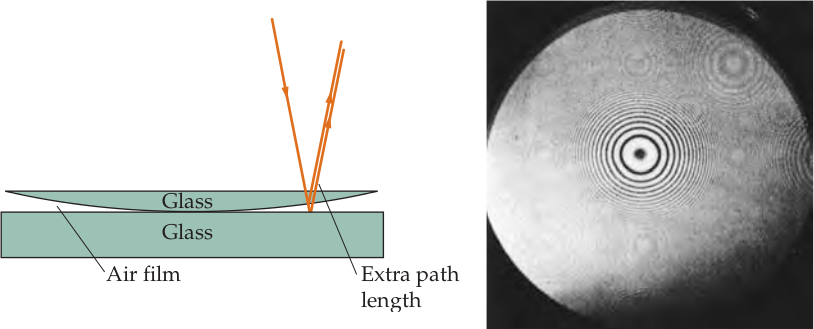
\includegraphics[width=0.9\textwidth]{images/6/62-newton.png}
\caption{Diagrama del muntatge dels anells de Newton. Es forma un anell quan augmentem el gruix de l'aire en $\pi$}
\end{figure}
\begin{figure}[H]
\centering
    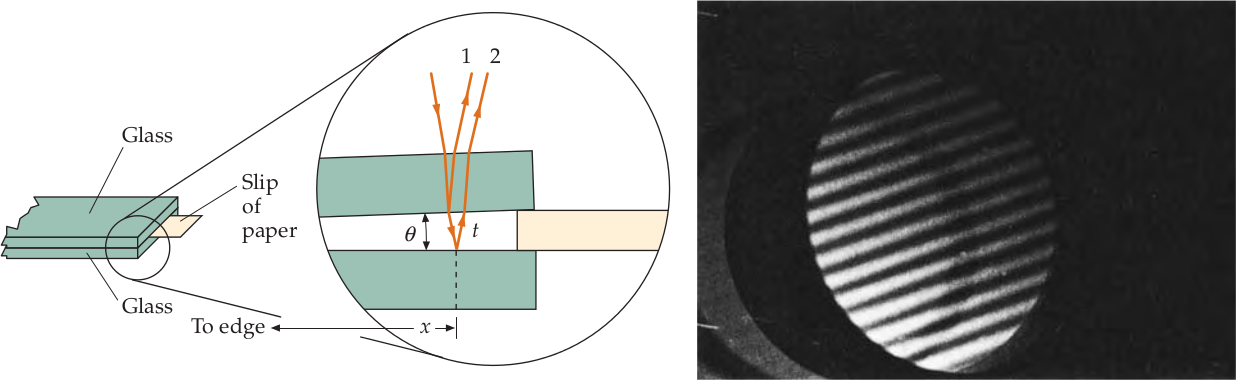
\includegraphics[width=\textwidth]{images/6/62-fizeau.png}
\caption{Diagrama del muntatge de les franges de Fizeau, que són equidistants}
\end{figure}

\subsubsection*{Pel·lícules anti-reflectants}
Són pel·lícules que per a certes longituds d'ona, la superposició d'ones harmòniques és destructiva, de manera que a fins pràctis no reflecteix. Les pel·lícules acostumen a tenir un índex de refracció de $n = 1.38$.

%----------------------------------------------------------------------------------------
\subsection{Divisió d'amplitud}
Un exemple és l'interferòmetre de Michelson.

%----------------------------------------------------------------------------------------
\subsection{Divisió de fronts d'ona}
\begin{figure}[H]
\centering
    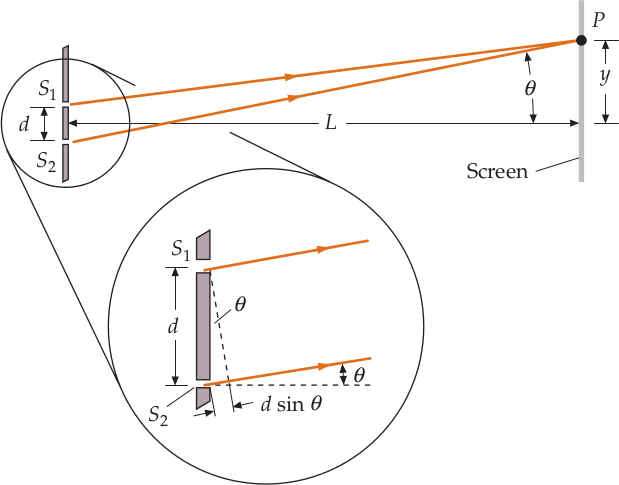
\includegraphics[width=0.6\textwidth]{images/6/64-int-doble.png}
\caption{Diagrama de la doble escletxa de Young}
\end{figure}
\subsubsection*{Patró d'interferència de dues escletxes}
\begin{itemize}
    \item Màxims: $\begin{gathered} \boxed{d \sin \theta_{m} = m \lambda} \end{gathered}, \quad m = 0, 1, 2 \dots$
    \item Mínims: $\begin{gathered} \boxed{d \sin \theta_{m} = (m - \frac{1}{2}) \lambda} \end{gathered}, \quad m = 1, 2, 3 \dots$
\end{itemize}
on $m$ és l'ordre d'interferència.

La diferència de fase ve donada per:
\begin{align} 
    \delta = d \sin \theta \frac{2 \pi}{\lambda} 
\end{align}
Podem relacionar la distància de les escletxes $L$ a la pantalla amb la distància $y_{m}$ a través de la pantalla:
\begin{align}
    \tan \theta_{m} = \frac{y_{m}}{L}
\end{align}
Llavors, per a angles petits $\tan \theta \approx \sin \theta$, i podem deduir:
\begin{align}
    \boxed{y_{m} = m \frac{\lambda L}{d}}
\end{align}

\subsubsection*{Càlcul de la intensitat}
\begin{align}
    \boxed{I = 4 I_{0} \cos^2 \left( \frac{1}{2} \delta \right)}
\end{align}

on $I_{0}$ és la intensitat de llum que arriba de cada escletxa i $\delta$ està relacionada amb la la posició a la pantalla.

%----------------------------------------------------------------------------------------
\subsection{Difracció}
\subsubsection*{Patró de difracció d'una escletxa}
\begin{figure}[H]
\centering
    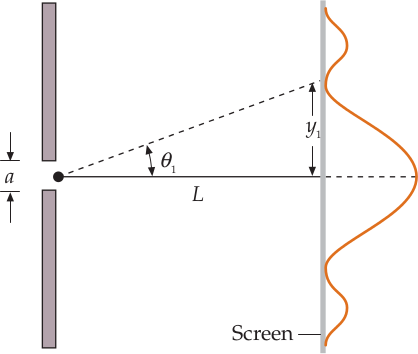
\includegraphics[width=0.4\textwidth]{images/6/65-dif-una.png}
\caption{Diagrama de difracció causada per una escletxa}
\end{figure}
\begin{itemize}
    \item Punts d'intensitat $I=0$: $\begin{gathered} \boxed{a \sin \theta_{m} = m \lambda} \end{gathered}, \quad m = 1, 2, 3 \dots$
\end{itemize}
Podem relacionar la distància de les escletxes $L$ a la pantalla amb la distància $y_{m}$ a través de la pantalla:
\begin{align}
    \tan \theta_{m} = \frac{y_{m}}{L}
\end{align}
Llavors, per a angles petits $\tan \theta \approx \sin \theta$, i podem deduir els punts d'intensitat zero:
\begin{align}
    \boxed{y_{m} = m \frac{\lambda L}{a}}
\end{align}

\subsubsection*{Patró d'interferència--difracció de dues escletxes}
\begin{figure}[H]
\centering
    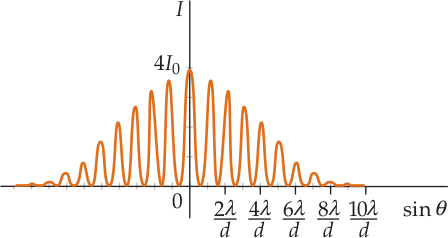
\includegraphics[width=0.6\textwidth]{images/6/65-int-dif-doble.png}
\caption{Diagrama de difracció causada per una escletxa}
\end{figure}
Al màxim central d'intensitat per difracció hi ha $N$ pics d'intensitat màxima per interferència. Com que el $m$-èsim màxim d'interferència és d'intensitat zero per difracció, tenim $m-1$ pics a cada banda del pic central. Llavors:
\begin{align}
    \boxed{N = 2(m-1) + 1 = 2m - 1}
\end{align}
Llavors, $m$ és l'ordre d'interferència tal que el primer mínim de difracció sigui igual a l'$m$-èsim màxim d'interferència:
\begin{align}
\begin{gathered}
    \sin \theta_{1} = \frac{\lambda}{a} = \sin \theta_{m} = m \frac{\lambda}{d}\\
    \Rightarrow \boxed{m = \frac{d}{a}} \Rightarrow \boxed{N = 2 \frac{d}{a} - 1}    
\end{gathered}
\end{align}

%----------------------------------------------------------------------------------------
\subsection{Ús de fasors per sumar ones harmòniques}
\subsubsection*{Patró d'interferència de tres o més fonts separades per la mateixa distància}
\subsubsection*{Patró d'interferència--difracció de múltiples escletxes}
\subsubsection*{Xarxa de difracció}

%----------------------------------------------------------------------------------------
\subsection{Difracció de Fraunhofer i Fresnel}
\begin{figure}[H]
\centering
    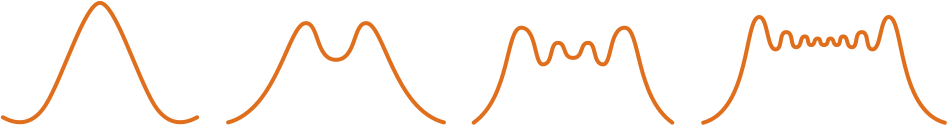
\includegraphics[width=\textwidth]{images/6/65-fraunhofer-fresnel.png}
\caption{El patró de difracció de Fraunhofer (paraxial) canvia gradualment al de difracció de Fresnel (no paraxial) quan apropem l'objecte a l'escletxa}
\end{figure}

\subsubsection*{Difracció i resolució}
La difracció a casa d'una obertura circular té importants implicacions per a la resolució de diferents instruments òptics. L'angle $\theta$ subtendit pel primer mínim difracció de Fraunhofer està relacionat amb la longitud d'ona i el diàmetre $D$ de l'obertura:
\begin{align}
    \boxed{\sin \theta = 1.22 \frac{\lambda}{D}}
\end{align}
En moltes aplicacions, l'angle $\theta$ és petit, llavors:
\begin{align}
    \theta \approx 1.22 \frac{\lambda}{D}
\end{align}
Dos focus puntuals subtendeixen un angle $\alpha$ amb l'obertura. Si $\alpha$ és molt major a $1.22 \lambda / D$ es veuran dos focus a l patró de difracció. Llavors per a una separació angular crítica $\alpha_{c}$ els dos focus se solaparan:
\begin{align}
    \boxed{\alpha_{c} = 1.22 \frac{\lambda}{D}}
\end{align}